\documentclass[svgnames]{article}
\usepackage{tikz,amsmath}

\usepackage{graphicx}
\pagestyle{empty}
\begin{document}

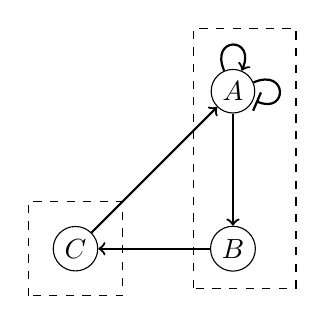
\begin{tikzpicture}[scale=1]
%%% Toy LRG
\node[shape=circle, draw, inner sep=2pt]  (A) at (2,2) {$A$};
\node[shape=circle, draw, inner sep=2pt]  (B) at (2,0) {$B$};
\node[shape=circle, draw, inner sep=2pt]  (C) at (0,0) {$C$};
\draw[dashed] (1.5,-0.5) rectangle (2.8,2.8);
\draw[dashed] (-0.6,-0.6) rectangle (0.6,0.6);
\draw[->,thick](A)--(B);
\draw[->,thick](A)..controls(1.7,2.7) and (2.3,2.7)..(A);
\draw[-|,thick,shorten >=1pt](A)..controls(2.7,2.3) and (2.7,1.7)..(A);
\draw[->,thick](B)--(C);
\draw[->,thick](C)--(A);

\end{tikzpicture}

\end{document}
